\documentclass[a4paper,11pt]{report}
\usepackage[T1]{fontenc}
\usepackage[utf8]{inputenc}
\usepackage{lmodern}
\usepackage[francais]{babel}
\usepackage{graphicx}
\usepackage{setspace}

\title{MonsterShip}
\author{Olivier \bsc{Boissard}, Kevin \bsc{Boulala},\\
Maxime \bsc{Dubois}, Antoine \bsc{Lavier}}
\date{Dernières modifications : \today}

\begin{document}

\maketitle
\tableofcontents

\chapter{Introduction}


\chapter{Contexte}


\chapter{Les objectifs}
    \section{Description générale du projet}
    C'est un jeu multijoueur par navigateur.\\

    Dans ce jeu le joueur contrôle et gère un vaisseau, le but étant de le faire grossir et prospérer.\\

    Pour se déplacer ou faire une action (attaquer, récolter des monstres), on utilise un système de points d'action qui se rechargent tous les jours.\\

    L’équipage du vaisseau est composé de petits monstres capables aussi bien de piloter le vaisseau en lui même, que de gérer les moteurs, utiliser les armes embarquées, etc. Pour faire prospérer son vaisseau, il faut utiliser son équipage comme une ressource de construction. Par exemple, le joueur souhaite avoir une arme plus puissante, le coût pour améliorer l’arme c’est de fusionner 2 membres de l’équipage avec cette arme. De même, le joueur peut fusionner des membres d'équipage avec le vaisseau, afin de l'agrandir pour pouvoir placer plus d'équipements (réacteurs, armes...).\\

    Pour améliorer son vaisseau, il faut explorer des planètes pour «recruter» d’autres membres. Lors du recrutement, le joueur aura le choix entre une action instantannée lui donnant accès à un certain nombre de monstres contre des points d'action, ou une action plus longue qui lui permet d'obtenir des monstres en fonction du temps resté à la surface. Dans ce dernier cas, le joueur est sujet aux attaques et il est par la même occasion plus vulnérable, mais il ne consomme aucun point d'action. Il faudra trouver le bon équilibre entre faire grossir son vaisseau pour pouvoir ajouter des équipements et augmenter la puissance de ces équipements, mais en gardant un équipage suffisamment important pour que chaque fonctionnalité du vaisseau puisse être exploitée à son plein potentiel.\\

    Les joueurs peuvent se rencontrer et organiser des batailles purement statistiques. Le vainqueur repartirait avec potentiellement quelques dégâts mineurs, mais surtout avec de nouveaux membres d’équipages. Le perdant, lui repartira un vaisseau endommagé, ayant perdu une partie de ses capacités, et un équipage réduit.\\

    \section{Les enjeux}
    L'objectif est de créer un jeu capable de concurrencer OGame.\\

    Pour cela, le jeu vise une clientèle large, allant des joueurs occasionnels, qui ne se connectent quelques fois par semaine, voire par mois, aux joueurs hardcore capables de passer plusieurs heures par jours à faire évoluer leur vaisseau.\\

    Pour cibler l'ensemble de cette clientèle, il est nécessaire d'avoir un mécanisme de jeu simple, avec une prise en main rapide. Pour cela, il n'existe qu'une seule ressource : l'équipage.\\

    Cette simplicité d'utilisation permettra également aux joueurs hardcores de mettre en place des stratégies au niveau du développement de leur vaisseau, afin de pouvoir vaincre les autres joueurs qui pourraient s'attaquer à eux.\\

\chapter{Définitions des éléments constituant le jeu}
    Le jeu est constitué d'un univers, dans lequel se trouvent des vaisseaux, appartenant aux joueurs.
    \section{L'univers}
        Le jeu est constitué de plusieurs éléments, chacun pouvant être utile au joueur, ou au contraire néfaste.
        \begin{description}
            \item[Etoiles] Ce sont des corps célestes extrêmements chauds et hostiles aux monstres et à leur vaisseau.
            \item[Planètes habitées] Ce sont des planètes où des monstres vivent. Le joueur peut y aller pour recruter de nouveaux membre d'équipage.
            \item[Planètes hostiles] Ce sont des planètes sur lesquels les monstres n'ont pu s'y installer pour diverses raisons, comme la température par exemple.
        \end{description}
      
    \section{Le vaisseau}
        Les vaisseaux sont constitués de différents modules, permettant de débloquer, ou d'améliorer les capacités du vaisseau.
        \begin{description}
            \item[Réacteur] C'est la pièce centrale permettant de créer de l'énergie pour alimenter les différents modules du vaisseau. Ainsi, s'il n'est pas suffisemment développé, le vaisseau ne pourra pas fonctionner à pleine puissance. Ce réacteur fournit de plus en plus d'énergie au fur et à mesure que les monstres fusionnent avec lui.
            \item[Poste de pilotage] C'est ici que l'on dirige le vaisseau.
            \item[Propulseur] C'est le module permettant de faire avancer le vaisseau. L'évolution de ce module permettra d'aller plus vite et plus loin.
            \item[Bouclier] Il permet d'avoir une protection globale qui se régénère avec le temps.
            \item[Radar] Ce module permet de détecter plus ou moins efficacement les éléments entourant le vaisseau (d'autres vaisseaux, des planètes, etc).
            \item[Arme] Il existe différents types d'armes selon l'objectif : certaines sont efficaces contre les boucliers, d'autres plus pour détruire la coque.
        \end{description}

        La quantité, et l'amélioration des modules sont limitées par la taille du vaisseau. Il est donc nécessaire d'agrandir régulièrement le vaisseau, en le fusionnant avec des monstres.\\

        Pour l'amélioration des modules, il sera nécessaire de fusionner des monstres avec les modules. Par exemple, nous avons un vaisseau avec un équipage de 10 monstres. Ils sont tous occupés à une tâche sauf 3. On utilisera un premier pour le fusionner avec le vaisseau afin de l'agrandir. Le second permettra alors de rajouter un propulseur, et le dernier sera affecté à l'entretien de ce nouveau module. Ainsi le vaisseau gagnera en vitesse.\\

\chapter{Expression fonctionnelle}
    \section{Graphe des intéractions}
        \begin{figure}[h]
            \begin{center}
                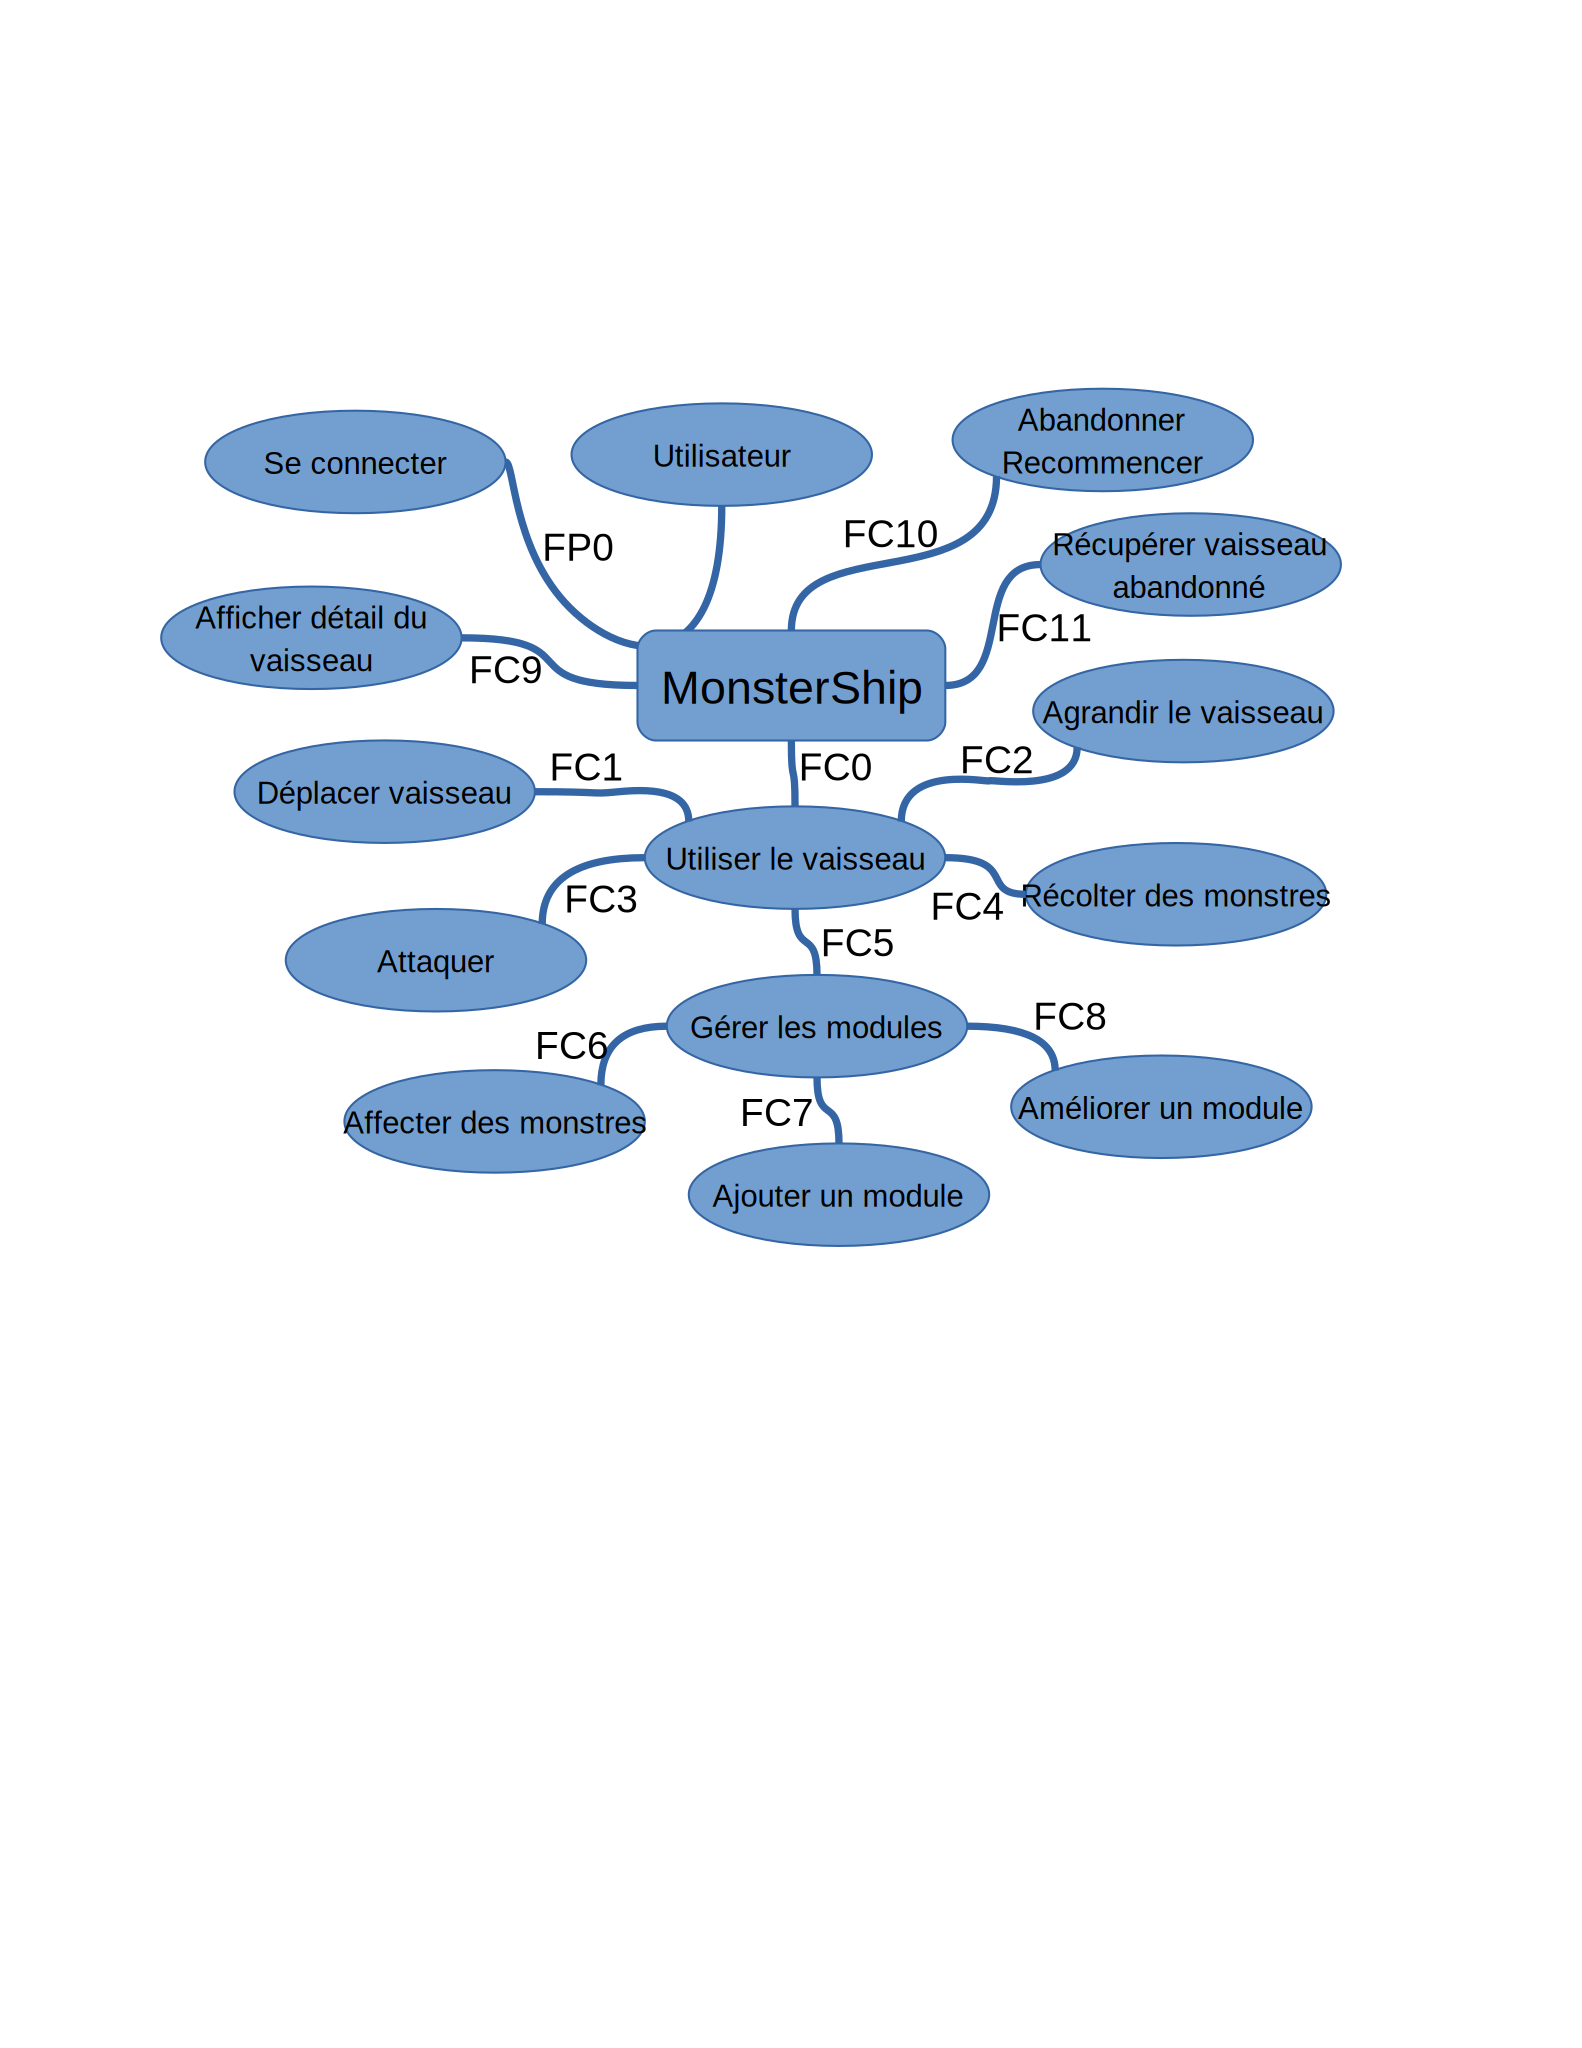
\includegraphics[width=\textwidth]{graphe_interactions.png}
                \caption{Graphe des intéractions}
                \label{fig:graphe_interactions}
            \end{center}
        \end{figure}

    \section{Les fonctions principales}
    % TODO FP0
    
    \section{Les fonctions secondaires}
    % TODO FC0 à FC11
    
\chapter{Maquette}


\chapter{Organisation et gestion du temps}


\end{document}
